\documentclass{article}
    \usepackage{amsmath}
    \usepackage{setspace}
    \usepackage{graphicx} %插入图片的宏包
    \usepackage{float} %设置图片浮动位置的宏包
    \usepackage{subfigure} %插入多图时用子图显示的宏包
   \usepackage{geometry}
    \geometry{a4paper,scale=0.7}
    \usepackage{pythonhighlight}
    \usepackage{longtable}
    


    %++++++++++++++++++++++++TITLE++++++++++++++++++++++
    \title{Linear Algebra in Neural Network}
    \author{CHEN Ming-yu\\2017200506032\\
    \and FENG Cheng-lin\\2017200506035\\
    \and YU Hong-ze\\2017200506034\\}
    \date{June 10 2018}
    
    %++++++++++++++++++++++++SETTING+++++++++++++++++++++
    \begin{document}
    \maketitle
    \begin{spacing}{2}
    \linespread{2}
    %+++++++++++++++++++++++BEGIN REPORT++++++++++++++++
    \section{Abstract}
    Today, one of the researches on aritificial intelligence is neural network. Sometimes people will find it hard to decide some situations, in other words, many decisions of human beings do not have quantified standards. Nevertheless, neural network can fulfill this job by training to get stabilized infrastructure.


    \noindent The problem we studied was converted into binary distribution with labeled wanted item ”1” and unwanted item “0”. Thus, after mapping the results within 0 to 1, the propagation outcome naturally becomes a binary digit. Then update each element in weight matrices by subtracting the gradients of cross entropy (the loss function). According to the figure above, the performance is acceptable after roughly 3000 steps.
    
    \section{Algorithmic Realization}

    To simplify the coding com
    \begin{figure}[H]
        \centering 
        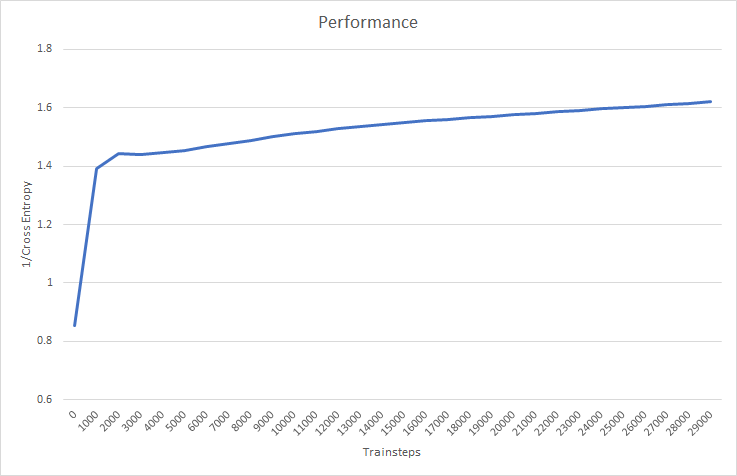
\includegraphics[width=1\textwidth]{Performance}
        \caption{Performance through out 30000 training stpes.}
        \end{figure}
  
    \noindent For
    

    \section{Conclusion}
 

    \section{Appendix}

  

   

    
    
    %++++++++++++++++++++BIBLIOGRAOHY+++++++++++++++++++++++
    \begin{thebibliography}{10}
   

    \end{thebibliography}

    \end{spacing}
    \end{document}